% Created 2020-02-24 Mon 16:13
% Intended LaTeX compiler: pdflatex
\documentclass[11pt]{article}
\usepackage[utf8]{inputenc}
\usepackage[T1]{fontenc}
\usepackage{graphicx}
\usepackage{grffile}
\usepackage{longtable}
\usepackage{wrapfig}
\usepackage{rotating}
\usepackage[normalem]{ulem}
\usepackage{amsmath}
\usepackage{textcomp}
\usepackage{amssymb}
\usepackage{capt-of}
\usepackage{hyperref}
\usepackage{minted}
\usepackage[top=0.8in, bottom=0.75in, left=0.625in, right=0.625in]{geometry}
\usepackage[english, russian]{babel}
\author{Sergey Makarov}
\date{\today}
\title{Учебный центр}
\hypersetup{
 pdfauthor={Sergey Makarov},
 pdftitle={Учебный центр},
 pdfkeywords={},
 pdfsubject={},
 pdfcreator={Emacs 26.3 (Org mode 9.3)}, 
 pdflang={Russian}}
\begin{document}

\maketitle
\tableofcontents

\section{Концептуальная модель UI}
\label{sec:org12254ae}
\subsection{Сценарии использования}
\label{sec:orge230e87}
\subsubsection{Получение списков обучающихся по курсам}
\label{sec:org8f7beba}
Чтобы получить список обучающихся на курсе, нужно авторизоваться как преподаватель и зайти
на страницу курса, который этот преподаватель ведёт. На этой странице будет список ссылок на
страницы обучающихся, записанных на курс.
\subsubsection{Получение истории обучения конкретного человека}
\label{sec:orgae300a9}
Чтобы получить историю обучения пользователя, нужно зайти на его страницу. Если обучающийся
разрешил отображение своей истории обучения, она будет представлена на этой странице.
\subsubsection{Получение списка всех преподавателей}
\label{sec:org46bf502}
Чтобы получить список всех преподавателей, нужно авторизоваться в качестве администратора курса,
зайти на страницу одного из администрируемых курсов, и перейти по ссылке составления расписания.
На этой странице будет ссылка на страницу со списком всех преподавателей.
\subsubsection{Получение списка преподавателей, ведущих данный курс}
\label{sec:org35b184f}
Список преподавателей, ведущих курс, приведён на странице курса, на которую можно попасть
с главной страницы, либо через форму поиска.
\subsubsection{Получение расписания преподавателя на заданный интервал времени}
\label{sec:orgbb33c16}
Получить расписание преподавателя можно зайдя на его страницу и нажав соответствующую кнопку.
\subsubsection{Получение расписания учащегося на заданный интервал времени}
\label{sec:org4430b2d}
Получить расписание учащегося можно зайдя на его страницу и нажав соответствующую кнопку.
\subsubsection{Составление расписания занятий для курса}
\label{sec:org6aa472c}
Для составления расписания занятий для курса нужно авторизоваться как администратор курса,
и выбрать курс из администрируемых или создать новый. На странице курса, на которую
пользователь попадает после этого, есть ссылка на страницу редактирования расписания, с
помощью которой и составляется расписание. После составления расписания, внесённые изменения
необходимо сохранить.
\subsubsection{Управление данными обучающихся}
\label{sec:org3c82cc7}
Авторизовавшись, обучающийся может редактировать данные о себе, хранимые в системе. Для
этого на его странице есть кнопка редактирования страницы, добавляющая к полям ФИО, почты,
биографии и контактов формы для установки новых значений соответствующих полей, и кнопку
применения изменений, фиксирующую изменения в базе. Кроме того, рядом с каждой формой при
редактировании данных отображается чекбокс, определяющий, нужно ли показывать данную
информацию на странице пользователя.
\subsubsection{Управление данными преподавателей}
\label{sec:org3a6d622}
Авторизовавшись, преподаватель может редактировать данные о себе, хранящиеся в системе. Для
этого на его странице есть кнопка редактирования страницы, добавляющая к полям ФИО, почты,
названия компании, биографии и контактов формы для установки новых значений соответствующих
полей, и кнопку применения изменений, фиксирующую изменения в базе. Кроме того, рядом с каждой формой при
редактировании данных отображается чекбокс, определяющий, нужно ли показывать данную
информацию на странице пользователя.
\subsubsection{Управление курсами}
\label{sec:org29f0853}
Авторизовавшись как администратор курса, пользователь может создавать новые курсы по ссылке
со страницы администратора курса, либо же перейти по ссылкам с этой же страницы к любому из
администрируемых курсов. На странице курса есть ссылка редактирования расписания курса. На
странице курса, помимо этого, есть кнопка редактирования описания курса, форма добавления
новых администраторов со списком уже добавленных, и чекбокс, определяющий, доступен ли курс
пользователям, отличным от администраторов.
\subsection{Страницы приложения}
\label{sec:org9dc8f07}
\subsubsection{Общие положения}
\label{sec:org3bbeee0}
В шапке каждой страницы приведены ссылки на главную страницу и страницу авторизации/выхода.
При переходе по ссылке на страницу выхода пользователь попадает на ту же страницу, если она
доступна неавторизованному пользователю, либо на главную.
\subsubsection{Главная страница}
\label{sec:org5440ca0}
На главной странице приведён список курсов в виде ссылок на них и поле
поиска курса. В результате поиска на главной будут отображаться только курсы, удовлетворяющие
условию поиска. Кроме того, на главной странице в шапке приведена ссылка на личную страницу
пользователя и кнопка выхода, если пользователь авторизован, и ссылки на страницы авторизации
и регистрации в противном случае. Большая часть функциональности приложения доступна только
после авторизации.
\subsubsection{Список преподавателей}
\label{sec:org50fb82e}
На этой странице приведены ссылки на страницы всех преподавателей, зарегистрированных в системе.
Кроме того, на этой странице есть кнопка поиска преподавателя, которая позволяет отфильтровывать
список.
\subsubsection{Страница обучающегося}
\label{sec:org6c1289c}
На странице обучающаяся приведено ФИО обучающегося, общая информация о нём, его контактные данные,
если обучающийся разрешил их отображение, и набор курсов, которые обучающийся проходил или
проходит, также если обучающийся разрешил отображение этих данных. Также на странице обучающегося
есть кнопка составления расписания, которая позволяет вывести расписание обучающегося на заданный
интервал. Если обучающийся авторизован, он может менять данные своей страницы и управлять их
доступностью, как сказано ранее. При нажатии на кнопку редактирования страницы возле полей ФИО,
общей информации и контактных данных появляются формы ввода новых значений и чекбокс,
определяющий, нужно ли отображать эти данные на странице. Изменения применяются после нажатия
кнопки сохранения изменений.
\subsubsection{Страница преподавателя}
\label{sec:orgdaab3d9}
На странице преподавателя отображается ФИО преподавателя, его контактная информация, если
включено отображение этой информации, название компании, в которой он работает,
и ссылки на курсы, занятия в которых он ведёт. Также на странице преподавателя есть кнопка
составления расписания, которая позволяет вывести расписание преподавателя на заданный интервал.
Если пользователь авторизован как преподаватель, он может управлять отображением контактной
информации на своей странице и редактировать данные на этой странице. При нажатии на кнопку редактирования страницы возле полей ФИО,
общей информации и контактных данных появляются формы ввода новых значений и чекбокс,
определяющий, нужно ли отображать эти данные на странице. Изменения применяются после нажатия
кнопки сохранения изменений.
\subsubsection{Страница администратора курса}
\label{sec:org3557bf5}
На этой странице предоставлен список ссылок на администрируемые пользователем курсы. Кроме
того, есть ссылка создания курса, с помощью которой создаётся новый курс, на страницу которого
администратор и попадает. По умолчанию созданный курс не виден никому, кроме администратора.
\subsubsection{Страница курса}
\label{sec:orga564a8a}
На странице курса приведено описание курса, диапазон дат его проведения, его интенсивность,
расписание и список ссылок на страницы преподавателей, ведущих курс.
Расписание представлено в виде списка дат и времени проведения занятий. В случае, если пользователь авторизован как
обучающийся, на странице есть также кнопка записи на курс, либо, если он уже записан, кнопка отмены записи.
Преподавателю, ведущему курс, доступен список ссылок на страницы обучающихся,
записанных на этот курс.
Если пользователь авторизован как администратор курса, он может редактировать расписание курса,
перейдя по соответствующей ссылке. Также есть кнопка редактирования описания курса, при нажатии
этой кнопки появляется форма для нового описания и кнопка сохранения изменений. Помимо этого, администратор курса
может назначать и отзывать других администраторов курса(для этого есть форма, куда пишется почта
добавляемого администратора), и показывать/скрывать курс от других пользователей(чекбокс).
\subsubsection{Страница редактирования расписания курса}
\label{sec:org49123b6}
На этой странице представлен набор занятий, проводимых во время курса. Можно изменять время
проведения курса, добавлять или удалять преподавателей, ведущих занятие, добавлять или удалять
занятия. Добавить преподавателя можно либо выбрав его из списка преподавателей, либо
посредством поиска. Внизу страницы есть кнопка фиксации изменений.
\subsubsection{Страница регистрации}
\label{sec:org3de71c3}
На странице регистрации можно зарегистрировать учётную запись для обучающегося или преподавателя.
Учётная запись администратора курса создаётся вручную из соображений безопасности.
Для регистрации обучающегося нужно предоставить электронную почту, логин и пароль, которые
будут использоваться для входа, ФИО обучающегося и опциональную биографическую информацию,
преподавателю дополнительно нужно предоставить название компании, в которой он работает.
\subsubsection{Страница авторизации}
\label{sec:orgd19dc19}
На странице авторизации можно войти как обучающийся, преподаватель, либо администратор курса.
Во всех трёх случаях авторизация происходит с помощью логина и пароля. После авторизации как
обучающийся, преподаватель или администратор курса пользователь попадает на страницу
обучающегося, преподавателя или администратора курса соответственно.
\subsection{Схема навигации между страницами}
\label{sec:org544dab5}
\begin{center}
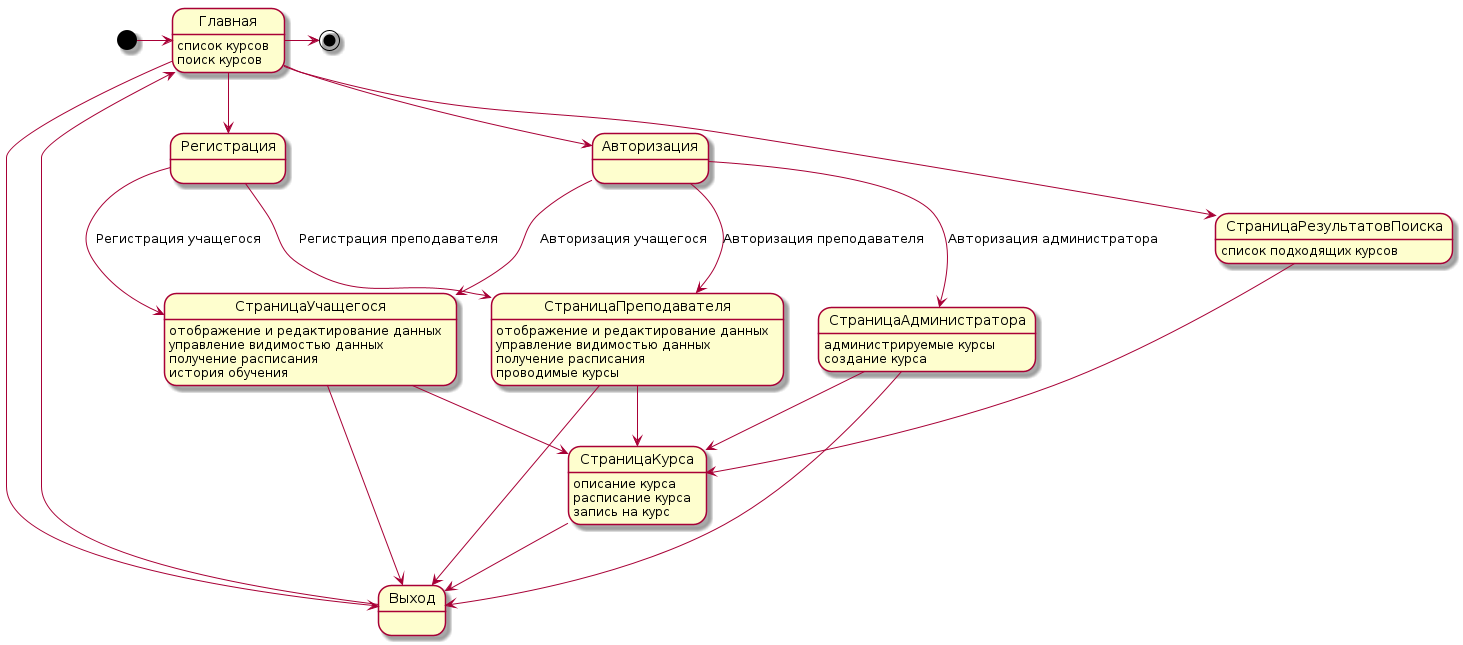
\includegraphics[width=.9\linewidth]{pages.png}
\end{center}

\section{База данных}
\label{sec:org530ff66}
\subsection{Схема базы данных}
\label{sec:org31d714b}
\begin{center}
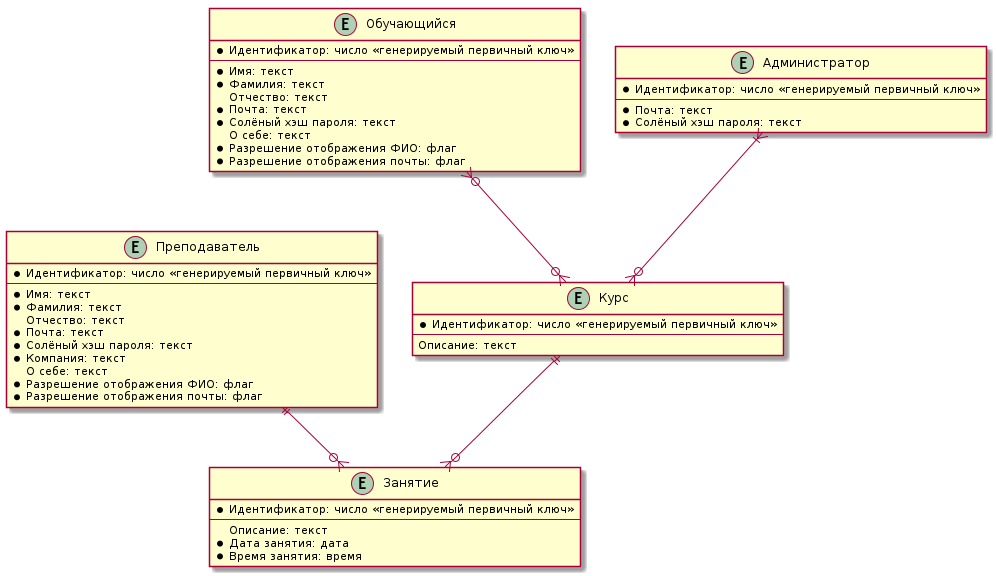
\includegraphics[width=.9\linewidth]{db.png}
\end{center}

\subsection{Скрипт создания базы данных}
\label{sec:orgb007b7b}
\begin{minted}[]{sql}
CREATE TABLE PUPIL (
  id serial PRIMARY KEY,
  firstname varchar(100) NOT NULL,
  lastname varchar(100) NOT NULL,
  patronymic varchar(100),
  mail varchar(254) NOT NULL,
  bio text,
  pass_hash varchar(64) NOT NULL,
  display_name boolean NOT NULL,
  display_mail boolean NOT NULL);

CREATE TABLE TEACHER (
  id serial PRIMARY KEY,
  firstname varchar(100) NOT NULL,
  lastname varchar(100) NOT NULL,
  patronymic varchar(100),
  company_name varchar(256) NOT NULL,
  mail varchar(254) NOT NULL,
  bio text,
  pass_hash varchar(64) NOT NULL,
  display_name boolean NOT NULL,
  display_mail boolean NOT NULL);

CREATE TABLE ADMINISTRATOR (
  id serial PRIMARY KEY,
  mail varchar(254) NOT NULL,
  pass_hash varchar(64) NOT NULL);

CREATE TABLE COURSE (
  id serial PRIMARY KEY,
  admin_id integer REFERENCES ADMINISTRATOR,
  description text);

CREATE TABLE LESSON (
  id serial PRIMARY KEY,
  description text,
  lesson_time timestamp NOT NULL,
  course_id integer REFERENCES COURSE,
  teacher_id integer REFERENCES TEACHER);

CREATE TABLE ADMIN_COURSE (
  id serial PRIMARY KEY,
  admin_id integer REFERENCES ADMINISTRATOR,
  course_id integer REFERENCES COURSE);

CREATE TABLE PUPIL_COURSE (
  id serial PRIMARY KEY,
  pupil_id integer REFERENCES PUPIL,
  course_id integer REFERENCES COURSE);
\end{minted}
\subsection{Скрипт заполнения базы данных}
\label{sec:org25d2f11}
\begin{minted}[]{sql}
SET DATESTYLE TO "DMY";

INSERT INTO PUPIL(firstname, lastname, mail, pass_hash, display_name, display_mail) VALUES('John',
'Doe', 'mail@example.com', 'fc4b5fd6816f75a7c81fc8eaa9499d6a299bd803397166e8c4cf9280b801d62c', TRUE, TRUE);
INSERT INTO PUPIL(firstname, lastname, mail, pass_hash, display_name, display_mail) VALUES('Jane',
'Doe', 'jdoe@bing.com', '8070d7385ec2439ca5d8d415c003cfde188803fc20d7f89291883a8ac4d61c9d', TRUE, FALSE);
INSERT INTO PUPIL(firstname, lastname, mail, pass_hash, display_name, display_mail) VALUES('Jimm',
'Craig', 'craig@gmail.com', '8bc4b88b1827764692b001ccc6696a23204a9fac043135ebad830b2af6fc8924', TRUE, FALSE);
INSERT INTO PUPIL(firstname, lastname, mail, pass_hash, display_name, display_mail) VALUES('Kate',
'Robinson', 'kate1984@bing.com', '25032daca58d5d3e677fe090e5be9ffd2b1a7ef68d585dd05c3dcacf3fce41c5', TRUE, TRUE);

INSERT INTO TEACHER(firstname, lastname, company_name, mail, pass_hash, display_name, display_mail) VALUES('Sergey',
'Kuznetsov', 'CS Center', 'mail@example.com', '6b3a55e0261b0304143f805a24924d0c1c44524821305f31d9277843b8a10f4e', TRUE, TRUE);
INSERT INTO TEACHER(firstname, lastname, company_name, mail, pass_hash, display_name, display_mail) VALUES('Oleg',
'Tarasov', 'CS Center', 'taroleg@gmail.com', '44e9385f53069b91d4afaa12f93a6e3353f83cc8f1db1f03093326416f32b98f', FALSE, FALSE);
INSERT INTO TEACHER(firstname, lastname, company_name, mail, pass_hash, display_name, display_mail) VALUES('Denis',
'Moskvin', 'CS Center', 'chrome@google.com', 'c942bc47f4c98e6bda9666c229c1dced88eec8ee73383d7c75de3dc21a3941f4', FALSE, FALSE);
INSERT INTO TEACHER(firstname, lastname, company_name, mail, pass_hash, display_name, display_mail) VALUES('Yegor',
'Bugayenko', 'CS Center', 'yegor256@gmail.com', '520ac20de525cd5a8c8c39c39b46b71a090ce968ff60f861737551d7bc2266d5', FALSE, TRUE);

INSERT INTO ADMINISTRATOR(mail, pass_hash) VALUES('nicolas@nmattia.com', '84eab5c7b4f0530a708350454e7f8ccaecde87cfbb9b1ed005da18685bf6776f');
INSERT INTO ADMINISTRATOR(mail, pass_hash) VALUES('robert@stuffwithstuff.com', 'c074d9749aa92d447e63edc69932ebf983b863685fe112646e7ae4314641e391');

INSERT INTO COURSE(description, admin_id) VALUES('Java programming', 1);
INSERT INTO COURSE(description, admin_id) VALUES('Databases', 2);

INSERT INTO LESSON(description, lesson_time, course_id, teacher_id) VALUES('Introduction',
'12-03-2020 16:20:00', 1, 2);
INSERT INTO LESSON(description, lesson_time, course_id, teacher_id) VALUES('Introduction',
'14-03-2020 16:55:00', 2, 3);
INSERT INTO LESSON(description, lesson_time, course_id, teacher_id) VALUES('Object-oriented programming',
'19-03-2020 16:20:00', 1, 4);
INSERT INTO LESSON(description, lesson_time, course_id, teacher_id) VALUES('History of databases',
'12-03-2020 16:55:00', 2, 4);

INSERT INTO ADMIN_COURSE(admin_id, course_id) VALUES(1, 1);
INSERT INTO ADMIN_COURSE(admin_id, course_id) VALUES(2, 2);

INSERT INTO PUPIL_COURSE(pupil_id, course_id) VALUES(1, 1);
INSERT INTO PUPIL_COURSE(pupil_id, course_id) VALUES(2, 2);
INSERT INTO PUPIL_COURSE(pupil_id, course_id) VALUES(3, 2);
INSERT INTO PUPIL_COURSE(pupil_id, course_id) VALUES(4, 1);
\end{minted}

Проверим заполнение таблиц:
\begin{minted}[]{sql}
SELECT * FROM PUPIL;
\end{minted}
\begin{minted}[]{sql}
SELECT * FROM TEACHER;
\end{minted}
\begin{minted}[]{sql}
SELECT * FROM ADMINISTRATOR;
\end{minted}

\begin{center}
\begin{tabular}{rll}
id & mail & pass\textsubscript{hash}\\
\hline
1 & nicolas@nmattia.com & 84eab5c7b4f0530a708350454e7f8ccaecde87cfbb9b1ed005da18685bf6776f\\
2 & robert@stuffwithstuff.com & c074d9749aa92d447e63edc69932ebf983b863685fe112646e7ae4314641e391\\
\end{tabular}
\end{center}

\begin{minted}[]{sql}
SELECT * FROM COURSE;
\end{minted}

\begin{center}
\begin{tabular}{rrl}
id & admin\textsubscript{id} & description\\
\hline
1 & 1 & Java programming\\
2 & 2 & Databases\\
\end{tabular}
\end{center}

\begin{minted}[]{sql}
SELECT * FROM LESSON;
\end{minted}

\begin{center}
\begin{tabular}{rllrr}
id & description & lesson\textsubscript{time} & course\textsubscript{id} & teacher\textsubscript{id}\\
\hline
1 & Introduction & 2020-03-12 16:20:00 & 1 & 2\\
2 & Introduction & 2020-03-14 16:55:00 & 2 & 3\\
3 & Object-oriented programming & 2020-03-19 16:20:00 & 1 & 4\\
4 & History of databases & 2020-03-12 16:55:00 & 2 & 4\\
\end{tabular}
\end{center}
\end{document}
